%%%%%%%%%%%%%%%%%%%%%%%%%%%%%%%%%%%%%%%%%%%%%%%%%%%%%%%%%%%%%%%%%%%%%%%%%%%%
%% Author template for Management Science (mnsc) for articles with no e-companion (EC)
%% Mirko Janc, Ph.D., INFORMS, mirko.janc@informs.org
%% ver. 0.95, December 2010
%%%%%%%%%%%%%%%%%%%%%%%%%%%%%%%%%%%%%%%%%%%%%%%%%%%%%%%%%%%%%%%%%%%%%%%%%%%%
\documentclass[mnsc]{informs3}
%\documentclass[mnsc,blindrev]{informs3}
%\documentclass[mnsc,nonblindrev]{informs3} % current default for manuscript submission

\OneAndAHalfSpacedXI
%%\OneAndAHalfSpacedXII % Current default line spacing
%%\DoubleSpacedXII
%%\DoubleSpacedXI

% If hyperref is used, dvi-to-ps driver of choice must be declared as
%   an additional option to the \documentclass. For example
%\documentclass[dvips,mnsc]{informs3}      % if dvips is used
%\documentclass[dvipsone,mnsc]{informs3}   % if dvipsone is used, etc.

% Private macros here (check that there is no clash with the style)
%%%%%%%% Linkage
\usepackage{xurl}
\usepackage{hyperref}
\hypersetup{colorlinks=true,citecolor=blue,urlcolor=blue}

%%%%%%%% Colored underline
\usepackage{ulem}
\usepackage{soul}
\makeatletter
    \newcommand{\coloruline}[2]{%
        \newcommand\temp@reduline{\bgroup\markoverwith
            {\textcolor{#1}{\rule[-0.5ex]{2pt}{0.4pt}}}\ULon}%
        \temp@reduline{#2}%
    }
    \newcommand{\coloruwave}[2]{%
        \UL@protected\def\temp@uwave{\leavevmode \bgroup 
        \ifdim \ULdepth=\maxdimen \ULdepth 3.5\p@
        \else \advance\ULdepth2\p@ 
        \fi \markoverwith{\textcolor{#1}{\lower\ULdepth\hbox{\sixly \char58}}}\ULon}
        \font\sixly=lasy6 % does not re-load if already loaded, so no memory drain.
        \temp@uwave{#2}%
    }
\makeatother

%%%%%%%% Algorithm
\usepackage{algorithm}
\usepackage{algorithmic}

%%%%%%%% Table, Figure and Diagram
%%%%%%%%%% Table
\usepackage{makecell}
\usepackage{tabularx}
\usepackage{array}
\usepackage{booktabs}
\usepackage{multirow}
%%%%%%%%%% Figure
\usepackage{float}
\usepackage{graphicx}
\usepackage{graphics}
\usepackage{caption,}
\usepackage{subcaption}
%%%%%%%%%% Diagram Figure
\usepackage{tikz}
\usetikzlibrary{arrows.meta, positioning}
\usepackage{varwidth}
%%%%%%%%%% Comments
\usepackage{comment}


% Natbib setup for author-year style
\usepackage{natbib}
 \bibpunct[, ]{(}{)}{,}{a}{}{,}%
 \def\bibfont{\small}%
 \def\bibsep{\smallskipamount}%
 \def\bibhang{24pt}%
 \def\newblock{\ }%
 \def\BIBand{and}%

%% Setup of theorem styles. Outcomment only one.
%% Preferred default is the first option.
\TheoremsNumberedThrough     % Preferred (Theorem 1, Lemma 1, Theorem 2)
%\TheoremsNumberedByChapter  % (Theorem 1.1, Lema 1.1, Theorem 1.2)
\ECRepeatTheorems

%% Setup of the equation numbering system. Outcomment only one.
%% Preferred default is the first option.
\EquationsNumberedThrough    % Default: (1), (2), ...
%\EquationsNumberedBySection % (1.1), (1.2), ...

% For new submissions, leave this number blank.
% For revisions, input the manuscript number assigned by the on-line
% system along with a suffix ".Rx" where x is the revision number.
\MANUSCRIPTNO{MS-0001-1922.65}


%%%%%%%%%%%%%%%%
\begin{document}
%%%%%%%%%%%%%%%%

% Outcomment only when entries are known. Otherwise leave as is and
%   default values will be used.
%\setcounter{page}{1}
%\VOLUME{00}%
%\NO{0}%
%\MONTH{Xxxxx}% (month or a similar seasonal id)
%\YEAR{0000}% e.g., 2005
%\FIRSTPAGE{000}%
%\LASTPAGE{000}%
%\SHORTYEAR{00}% shortened year (two-digit)
%\ISSUE{0000} %
%\LONGFIRSTPAGE{0001} %
%\DOI{10.1287/xxxx.0000.0000}%

% Author's names for the running heads
% Sample depending on the number of authors;
% \RUNAUTHOR{Jones}
% \RUNAUTHOR{Jones and Wilson}
% \RUNAUTHOR{Jones, Miller, and Wilson}
% \RUNAUTHOR{Jones et al.} % for four or more authors
% Enter authors following the given pattern:
%\RUNAUTHOR{}

% Title or shortened title suitable for running heads. Sample:
% \RUNTITLE{Bundling Information Goods of Decreasing Value}
% Enter the (shortened) title:
\RUNTITLE{Bayesian Structural Inference for Dynamic Crowdsourcing Contests}

% Full title. Sample:
% \TITLE{Bundling Information Goods of Decreasing Value}
% Enter the full title:
\TITLE{Bayesian Structural Inference for Dynamic Crowdsourcing Contests}

% Block of authors and their affiliations starts here:
% NOTE: Authors with same affiliation, if the order of authors allows,
%   should be entered in ONE field, separated by a comma.
%   \EMAIL field can be repeated if more than one author
\ARTICLEAUTHORS{%
\AUTHOR{Jussi Keppo}
\AFF{NUS Business School and Institute of Operations Research and Analytics\\
	National University of Singapore, Singapore\\
	\EMAIL{keppo@nus.edu.sg}} %, \URL{}}
\AUTHOR{Linsheng Zhuang}
\AFF{Institute of Operations Research and Analytics\\
	National University of Singapore, Singapore\\
	\EMAIL{linsheng.z@u.nus.edu}}
% Enter all authors
} % end of the block

\ABSTRACT{%
...
% Enter your abstract
}%

% Sample
%\KEYWORDS{deterministic inventory theory; infinite linear programming duality;
%  existence of optimal policies; semi-Markov decision process; cyclic schedule}

% Fill in data. If unknown, outcomment the field
\KEYWORDS{Digital Economy, Data Protection Regulation, Innovation Contest} 
%\HISTORY{......}

\maketitle
%%%%%%%%%%%%%%%%%%%%%%%%%%%%%%%%%%%%%%%%%%%%%%%%%%%%%%%%%%%%%%%%%%%%%%

% Samples of sectioning (and labeling) in MNSC
% NOTE: (1) \section and \subsection do NOT end with a period
%       (2) \subsubsection and lower need end punctuation
%       (3) capitalization is as shown (title style).
%
%\section{Introduction.}\label{intro} %%1.
%\subsection{Duality and the Classical EOQ Problem.}\label{class-EOQ} %% 1.1.
%\subsection{Outline.}\label{outline1} %% 1.2.
%\subsubsection{Cyclic Schedules for the General Deterministic SMDP.}
%  \label{cyclic-schedules} %% 1.2.1
%\section{Problem Description.}\label{problemdescription} %% 2.

% Text of your paper here


\section{Introduction}

\begin{itemize}
\item Kaggle\footnote{\url{https://www.kaggle.com}} ...
\item Meta-kaggle dataset \cite{megan_risdal_timo_bozsolik_2022}. 
\end{itemize}

\subsection{Related Literature}

This paper focuses on the two players innovation contest with a continuous time  where the players’ relative position is public information throughout the game.
This is closely related to tug-or-war contest, which, to our knowledge, was first formally given by \citet{Harris1987Race} as a one-dimensional simplification of the multi-stage R\&D race. 
The output processes are model by Brownian motions drifted with effort inputs, which is followed by \cite{budd1993model} who model the state of a dynamic competition of two innovative duopoly firms by a Brownian motion drifted by the effort gap, and solve the equilibrium approximately. 
Furthermore, \citet{Moscarini2011Contest} model the tug-of-war state as the gap of the two outputs directly, and draw an analytical equilibrium of the pure strategies. 

...

Information disclosure in contest - \cite{Bimpikis2019Contest}. 

...

Closest paper - \cite{ryvkin2022fight}.

...




\section{The Model}\label{contest-theory}

% Effort, Output and Gap
Two players, $i$ and $j$, compete for a prize $\theta>0$ in a contest. 
Winner gets the prize and loser gets nothing. 
The contest starts at time zero. 
At every time $t\ge0$, the representative player $i$ chooses an effort level $q_{i,t}$ and burdens a quadratic cost $C_i(q_{i,t}) = c_i q_{i,t}^2/2$, with a lower $c_i$ corresponding to higher ability. 
Denoted by $y_t$ the \textit{output gap} of player $i$ and $j$ at time $t$, driven by
\begin{equation}\label{eq-state-dynamics}
	dy_t = (q_{i,t}-q_{j,t})dt + \sigma dW_t
\end{equation}
where $W_t$ is a Brownian motion and $\sigma>0$ measures the innovation risk.

The contest is equipped with a submission system that allows participants to upload their algorithms at any time and receive immediate feedback. 
For simplicity, we further assume that agents submit their intermediate results whenever they make progress. 
This setup enables the contest organizers to monitor all players’ progress $x_{i,t}$ and $x_{j,t}$ in real time. 
Moreover, the true output level, evaluated by the system, is only known by the game designer but not the two players. 
% Signal
At any time $t>0$, the contest designer emits a \textit{public} signal of the real output gap $y_t$. 
The signal is ambiguous and the game holder controls the ambiguity. 
The dynamic of signal is  
\begin{equation}\label{signal}
	dZ_{t} = y_{t}dt + \frac{dB_{t}}{\sqrt{\lambda}} 
\end{equation}
where $B_{t}$ is standard Brownian motion independent with $(W_{i,t})$ and $(W_{j,t})$, and the parameter $\lambda$ is set by the game holder to control the precision of signal. 
The larger the $\lambda$, the more accurate the signal would be. 

% Bayesian Player
The information set of both players at time $t \ge 0$ is  $I_{t} \equiv \{Z_{s} : 0\le s \le t\}$. 
Player $i$ estimates the unknown output gap $y_t$ based on the information set $I_t$. 
Let $\tilde{y}_t \equiv E(y_{t}|I_t)$ be the estimated output gap and $S_t \equiv E[(\tilde{y}_{t}-y_{t})^2|I_t]$ be the estimation variance. 
According to Chapter 1.2 of \citet{Bensoussan1992Control}, \textit{Kalman-Bucy filter} gives the dynamics of $\tilde{y}_{t}$ and $S_{t}$, 
\begin{align}
	d\tilde{y}_{t} &= (q_{i,t}-q_{j,t})dt + \lambda S_{t}(dZ_{t}-\tilde{y}_{t}dt) 
	\label{filtered-x}\\
	\frac{dS_{t}}{dt} &= \sigma^2 - \lambda S_{t}^2
	\label{filtered-S}
\end{align} 
Hence, the conditional distribution $y_{t}|I_t\sim\mathcal{N}(\tilde{y}_{t},S_{t}|I_t)$ is fully captured by the mean $\tilde{y}_{t}$ and variance $S_{t}$. 
If $\lambda = 0$, we have $S_t = S_0+\sigma^2t$, i.e., the estimation variance is increasing in time linearly. 
If $\lambda > 0$, the solution of (\ref{filtered-S}) is
\begin{equation}\label{S-evolution} 
	S_t = 
	\begin{cases}
        \bar{S} \cdot \tanh\left\{t\cdot\sigma\sqrt{\lambda} +  \tanh^{-1}\left(S_0\big/\bar{S}\right)\right\} & \text{if } S_0 < \bar{S} \\
        \bar{S} & \text{if } S_0 = \bar{S} \\
        \bar{S} \cdot \coth\left\{t\cdot\sigma\sqrt{\lambda} +  \coth^{-1}\left(S_0\big/\bar{S}\right)\right\} & \text{if } S_0 > \bar{S} 
	\end{cases}
\end{equation}
Specifically, $\bar{S} = \sigma / \sqrt{\lambda}$ when $\lambda>0$ and $\bar{S} = \infty$ when $\lambda = 0$. 
Please refer to Appendix~\ref{app-S-equ} for the derivations. 
Figure~\ref{fig-S-evol} shows the evolution of $S_t$ in time: estimation variance $S_t$ converges to \textit{steady state} $\bar{S}$ as time goes by regardless of the starting estimation variance. 
For simplicity, we henceforth assume that $S_0 = \bar{S}$, hence $S_t\equiv \bar{S}$. 

\begin{figure}[!ht]
	\centering
	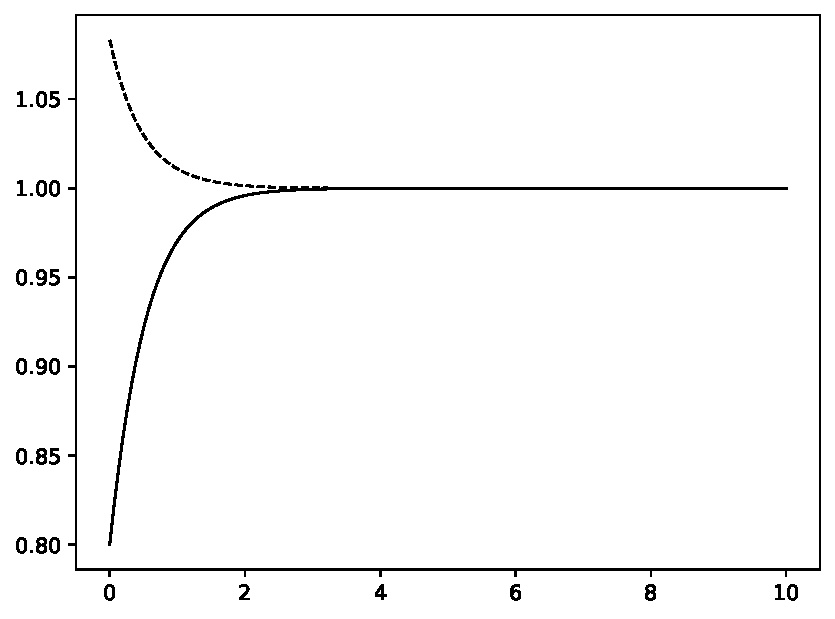
\includegraphics[scale=0.6]{figure_S_evolve.pdf}
	\caption{The evolution of $S_t$ in time $t$, given that $\lambda = 1$ and $\sigma = 1$.} \label{fig-S-evol}
\end{figure}



% Contest Deadline
Following \cite{ryvkin2022fight}, let's consider a dynamic contest with a fixed deadline. 
Suppose the contest is terminated when time $t=T>0$. 
Since the steady state estimation variance $\bar{S}$ is fixed as displayed above, the state of the game is fully characterized by a tuple $(\tilde{y}_t, t)$. 
At any time $0\le t<T$, player $i$ optimizes her effort level $q_{i,\tau}$ in the remaining contest period $\tau\in[t, T)$ according to the following optimization problem, 
\begin{equation}\label{v-def}
	V^i(\tilde{y}_{t}, t ; q_{j,t},\Theta_i) = \max_{\{q_{i,\tau}\}^T_{\tau=t}} 
	\mathbb{E}\left( \theta\cdot1_{\tilde{y}_T>0} - \int^T_tC_i(q_{i,\tau})d\tau \bigg|I_t\right) 
\end{equation}
where $\Theta_i \equiv\{\theta, \lambda, \sigma, c_i\}$, subject to constraints (\ref{filtered-x}), (\ref{filtered-S}) and $q_{i,\tau}\ge0$ for all $\tau\in[t,T)$.
The optimization problem for player $j$ is just symmetric to that of player $i$ as $V^j(\tilde{y}_t, t) = V^i(-\tilde{y}_t, t)$. 
The corresponding Hamilton-Jacobi-Bellman (HJB) equation for player $i$ is 
\begin{equation*}
0 = \max_{q_{i,t}\ge0}\left[-\frac{c_iq_i^2}{2} + V^i_{y}\cdot\left(q_{i,t}-q_{j,t}\right)+V^i_t + \frac{V^i_{yy}}{2}\lambda \bar{S}^2\right]
\end{equation*}
By definition, we have $\lambda \bar{S}^2 = \sigma^2$. 
Under the assumption of inner solution, we plug into the first order conditions $q_{i,t} = V^i_y/c_i$ and $q_{j,t} = -V^j_y/c_j$, we have the system of equations
\begin{equation*}
\begin{aligned}
\frac{1}{2c_i}(V^i_y)^2 + \frac{1}{c_j}V^i_yV^j_y + V^i_t + V^i_{yy}\frac{\sigma^2}{2} = 0\\
\frac{1}{2c_j}(V^j_y)^2 + \frac{1}{c_i}V^j_yV^i_y + V^j_t + V^j_{yy}\frac{\sigma^2}{2} = 0
\end{aligned}
\end{equation*}
subject to boundary conditions $V^i(-\infty, t) = 0$, $V^i(+\infty, t) = \theta$, $V^j(-\infty, t) = \theta$, $V^j(+\infty, t)=0$, $V^i(\tilde{y}_T, T) = \theta \cdot 1_{\tilde{y}_T > 0}$ and $V^j(\tilde{y}_T, T) = \theta \cdot 1_{\tilde{y}_T < 0}$. 


The Nash equilibrium is summarized in the following lemma. 
We include a simplified version of the proof in the appendix: 

\begin{lemma}[\citealt{ryvkin2022fight}]
In the Markov perfect equilibrium, the players’ efforts in state $m_{i(j)}(\tilde{y}_t, t) :\mathbb{R}\times[0, T)\to\mathbb{R}_+$ are given by
\begin{equation}\label{eq-equilibrium-effort}
m_{i(j)}(\tilde{y}_t, t) = \frac{e^{-z^2/2}}{\sqrt{2\pi\sigma^2(T-t)}}\cdot \frac{\sigma^2}{2}\left[\gamma(\rho_{i}) + \gamma(\rho_{j})\right]\left[1-\rho(z)^2\right]\left[1 \pm \rho(z)\right]
\end{equation}
where $z = \tilde{y}_t / (\sigma\sqrt{T-t})$, $\rho(z) = \gamma^{-1}\left(\Phi(z)\left[\gamma(\rho_{i})+\gamma(\rho_{j})\right]-\gamma(\rho_{j})\right)$ and 
\begin{equation*}
\gamma(u) = \frac{u}{1-u^2} + \frac{1}{2}\ln\frac{1+u}{1-u},\quad u\in(-1,1)
\end{equation*}
\begin{equation*}
\rho_{i} = \frac{e^{w_{i}}+e^{-w_{j}}-2}{e^{w_{i}}-e^{-w_{j}}},
\quad
\rho_{j} = \frac{e^{w_{j}}+e^{-w_{i}}-2}{e^{w_{j}}-e^{-w_{i}}},
\quad
w_{i(j)} = \frac{\theta}{\sigma^2 c_{i(j)}}.
\end{equation*}
\end{lemma}

The variables $w_{i(j)}$ represent the abilities of two players, while $\rho_{i(j)}$ normalizes $w_{i(j)}$ into the interval $(-1, 1)$. 
It is not hard to see that $\gamma(\cdot)$ is strictly increasing on $(-1,1)$, ranging from $-\infty$ to $+\infty$. 
Moreover, the equilibrium effort $m_{i(j)}$ can be represented to the product of $\phi(y; 0, \sigma^2(T-t))$, the probability density of normal distribution with mean zero and variance $\sigma^2(T-t)$ at the state $y$ and an amplitude factor that only depends on the composite variable $z$. 

To Do: Contest Design Rules

\begin{proposition}
...
\end{proposition}




\section{Estimation Framework}\label{sect-bayes-framework}

In this section, we describe the estimation procedure. 
We first outline the data generation process, establishing the connection between the empirical data and the theoretical model discussed previously.
Then, we introduce a structural estimation method using Bayesian framework.

\subsection{Data-Generating Process}

For each Kaggle contest, the observable data from the Meta-Kaggle dataset can be categorized into three main components:

%% Data: Contest setting
The first component consists of essential contest details, including the contest duration, prize structure, information disclosure policy, and other governing rules.
%%%% Prob 1
Contrary to the assumptions of our model, a typical contest usually involves multiple teams rather than just two.
In Section~\ref{sec-kaggle-application}, we focus on the two strongest participants in each contest for analysis; further discussion on this choice is provided in Section~\ref{sect-extension}.
%%%% Prob 2
Furthermore, many contests adopt complex prize structures, offering multiple awards rather than following a winner-takes-all format.
In Section~\ref{sec-kaggle-application}, we begin by selecting contests that offer a single prize awarded in USD.
Extensions to more general prize structures are presented in Section~\ref{sect-extension}.

%% Data: Submissions
The second component captures the submission events of each player $i$ to the system, denoted by the sequence $\{\hat{t}^i_k\}_{k=1}^{N_i}$.
Here, $N_i$ represents for the total number of submissions by player $i$, and $t$ represents for the time of each submission. 
We understand the submission events of player $i$ and $j$ as two conditional independent inhomogeneous Poisson processes, driven by the intensity functions $\tau_i(t)$ and $\tau_j(t)$.\footnote{That is, given the intensity functions $\tau_i(t)$ and $\tau_j(t)$, the submission events $\{\hat{t}^i_k\}_{k=1}^{N_i}$ and $\{\hat{t}^j_k\}_{k=1}^{N_i}$ are mutually independent.}
Then, during any time interval $\mathcal{S}$ of the contest duration $\mathcal{T}$, the Poisson arrival rate of submissions of the representative player $i$ is given by $\int_{s\in\mathcal{S}}\tau_i(s)ds$. 
We assume the submission intensity $\tau_i(t)$ is proportional to the effort level $m_i(\tilde{y}_t, t)$. More specifically, 
\begin{equation}\label{eq-model-intensity}
\tau_i(t) = r \cdot m_i(\tilde{y}_t, t)
\end{equation}
where $r>0$ is the ratio of submission intensity to effort level, serving as a tuning parameter for numerical stability. 


%% Data: Leaderboard
The third component of the contest data is the \textit{public} and \textit{private} leaderboard that records the real-time rankings and scores of each participant, denoted by $\hat{x}^{i(j)}_t$ and $x^{i(j)}_t$. 
In Kaggle competitions, most organizers deliberately disclose only a subset of the full dataset to participants to mitigate the risk of overfitting. 
The proportion of the released data is generally known to all participants. 
The public leaderboard is updated upon each submission, using only the released portion of the dataset; as a result, the signals it provides are inherently noisy.
In addition to the public leaderboard, most competitions hosted on Kaggle also maintain a private leaderboard, where organizers evaluate the true predictive performance of participants’ models using the full dataset.
The true output gap $y_t := x^i_t - x^j_t$ is generated according to equation (\ref{eq-state-dynamics}).
It is observable only by the game designer during the contest and becomes available from the Meta-Kaggle dataset after the contest concludes. 
Furthermore, we interpret the difference in scores between $i$ and $j$ displayed on the public leaderboard as the signal $Z_t$ defined in (\ref{signal}), released by the contest organizer. 
Specifically, let's denote $\hat{y}_t = \hat{x}^i_t - \hat{x}^j_t$ the gap between displayed scores, and interpret it as the signal intentionally released by the contest organizer: 
\begin{equation}\label{eq-model-signal}
dZ_t = \hat{y}_tdt
\end{equation}
Combining (\ref{signal}) with (\ref{eq-state-dynamics}), the observed real-time gap $\hat{y}_t$ on leaderboard evolves as 
\begin{equation}\label{eq-leaderboard-gap}
\hat{y}_t = y_t + \frac{1}{\sqrt{\lambda}}\frac{dB_t}{dt} = \int^t_0\left[m_i(\tilde{y}_t, s) - m_j(\tilde{y}_t, s)\right]ds + \sigma W_{t} + \frac{\xi_t}{\sqrt{\lambda}}
\end{equation}
where the term $\sigma W_t$ captures the accumulated innovation shock, $\lambda$ governs the signal precision and $\xi_t$ is a white noise with $\mathbb{E}(\xi_t\xi_s) = \delta(t-s)$. 
In practise, we approximately assume that $\xi_t \approx (B_{t+\Delta} - B_t)/\Delta$ where $\Delta$ is a small time interval. 

% Source of Noise 2
Beyond the uncertainty introduced by partial data disclosure, a second source of signal noise arises from the timing of leaderboard updates: 
rankings are refreshed only after model submissions, leaving the leaderboard uninformative during periods without new submissions.
It should be noted that such lag would significantly bias our model estimates only if participants strategically timed their submissions.
Although such strategic behaviour is theoretically possible, we abstract from it in this study.
We assume that each submission follows a period of substantive effort, allowing the leaderboard rankings to broadly reflect the relative performance of algorithms based on the publicly available data.

% tilde{y}_t
It is important to recognize that the generation of $y_t$ and $\hat{y}_t$ is inherently tied to the players’ strategic interactions, as it depends on their estimates of the underlying state, $\tilde{y}_t$. 
In turn, $\tilde{y}_t$ evolves dynamically based on $\hat{y}_t$, since players continually update their beliefs in response to observed data. 
As a result, the generation of $y_t$, $\hat{y}_t$ and $\tilde{y}_t$ proceeds jointly.
By equations (\ref{filtered-x}) and (\ref{eq-model-signal}), the estimated gap $\tilde{y}_t$ as perceived by the two players, is determined by the following stochastic differential equation:
\begin{equation}\label{eq-fintered-y-update}
d\tilde{y}_{t} = \left[m_i(\tilde{y}_t, t) - m_j(\tilde{y}_t, t)\right]dt + \sqrt{\lambda}\sigma(\hat{y}_t-\tilde{y}_{t}) dt
\end{equation}
with initial condition $\tilde{y}_0 = \mu_0$, where $\mu_0$ can be interpreted as the prior mean of the initial true state $y_0$.

We denote the set of unknown parameters by $\Theta := \{c_i, c_j, \sigma, \lambda, \mu_0\}$.
Once $\Theta$ is specified, the data-generating processes for $(y_t)$, $(\hat{y}_t)$, and $(\tilde{y}_t)$ are fully defined by equations (\ref{eq-state-dynamics}), (\ref{eq-leaderboard-gap}), and (\ref{eq-fintered-y-update}), although their realized trajectories remain stochastic.


\subsection{Bayesian Estimation Framework}

Our objective is to develop a Bayesian framework for inferring the unknown parameter set $\Theta := \{ c_i, c_j, \sigma, \lambda, \mu_0 \}$ using the data introduced above.

First of all, we assume that time is discretized into uniform intervals of length $\Delta$.
By definition, the likelihood function corresponding to the submission times of player $i$, $\{t^i_k\}_{k=1}^{N_i}$, is given as follows (a symmetric formulation applies to player $j$):
\begin{equation}\label{eq-ihpp-prob}
p\left(\{\hat{t}^i_k\}_{k=1}^{N_i} | \tau_i, \Theta\right) = \exp\left\{-\int_{s\in\mathcal{T}}\tau_i(s)ds\right\}\prod_{k=1}^{N_i}\tau_i(\hat{t}^i_k)
\end{equation}
where $\tau_i$ is defined in (\ref{eq-model-intensity}) with the tuning parameter $r$ exogenously specified. 
Since time is discretized, the integrals on the left-hand side can be approximated by finite sums.

Next, suppose the public leaderboard gaps $\hat{y}_t$ is sampled at time points $(t_1, t_2, ..., t_N)$, yielding observations $\{\hat{y}_{t_k}\}^N_{k=1}$. 
Let $t_0 = 0$ and suppose the initial gap satisfies $y_0 = 0$. 
Then, according to the assumed data-generating process of $\hat{y}_t$ in (\ref{eq-leaderboard-gap}), the corresponding likelihood function is
\begin{equation}\label{eq-obs_gap-prob}
p\left(\{\hat{y}_{t_k}\}_{k=1}^N | \{\hat{t}^{i(j)}_k\}_{k=1}^{N_{i(j)}}, m_i, m_j, \Theta\right) = 
\phi\left(\{\hat{y}_{t_k}\}_{k=1}^N | \left\{\mu_k\right\}^N_{k=1}, \Sigma_y+\frac{I_N}{\Delta\lambda}\right)
\end{equation}
where $\mu_k = \int_{0}^{t_{k}}m_i(\tilde{y}_s, s) - m_j(\tilde{y}_s, s)ds$ and $\Sigma_y(i, j) = \sigma^2\min(t_i,t_j)$. 
Moreover, let $N = N_i + N_j$, indicating that the public leaderboard is updated once a new submission occurs. 

%% Note: exclude y_t in likelihood
It's worthwhile noting that, although the trajectory of private leaderboard $y_t$ is available ex post from the Meta-Kaggle dataset, we deliberately exclude it from the likelihood function. 
In our framework, agents form beliefs about $y_t$ based solely on $\hat{y}_t$, and their actions are driven by these beliefs. 
Conditioning on the realized values of $y_t$ in estimation would effectively bypass the agent’s informational constraints and undermine the role of $\lambda$ in shaping belief formation. 
More importantly, it would prevent us from evaluating whether the proposed model—when given only the information actually available to agents—can recover the true data-generating process. 
Treating $y_t$ as latent therefore preserves the integrity of the causal structure and enables meaningful model validation after estimation (see Figure~\ref{kaggledata-diagram}).

%% Approximation
To evaluate the likelihood functions (\ref{eq-ihpp-prob}) and (\ref{eq-obs_gap-prob}), we must first compute the equilibrium trajectories of both the perceived output gap $(\tilde{y}_t)$ and the effort levels $(m_i(\tilde{y}_t, t), m_j(\tilde{y}_t, t))$, as implied by equations (\ref{eq-equilibrium-effort}) and (\ref{eq-fintered-y-update}). 
Importantly, the construction of $\tilde{y}$ and the effort functions $m_i$ and $m_j$ depends on the underlying (unobserved) parameters $c_i$, $c_j$, $\sigma$ and $\lambda$, which are themselves subject to estimation.

Once these parameters are specified, the equilibrium paths of the perceived output gap $(\tilde{y}_t)$ and the corresponding effort levels $(m_i(\tilde{y}_t, t), m_j(\tilde{y}_t, t))$ can be deterministically computed. 
However, evaluating $m_{i(j)}(\tilde{y}_t, t)$ via equation~(\ref{eq-equilibrium-effort}) requires numerically approximating the inverse function $\gamma^{-1}$, which poses challenges for the use of gradient-based Markov Chain Monte Carlo (MCMC) sampling methods, such as Hamiltonian Monte Carlo (HMC, \citealt{neal1996bayesian}, \citealt{neal2011mcmc}, \citealt{betancourt2017conceptual}) and the No-U-Turn Sampler (NUTS, \citealt{hoffman2014NUTS}).
Hence, we approximate this inverse function with an analytical form:
\begin{equation}\label{eq-invgamma-approx}
\gamma^{-1}(x) \approx \frac{2}{\pi}\arctan(a \cdot x)
\end{equation}
where $a$ is around 0.947 by minimizing the 1-norm of the difference between the numerical inverse of $\gamma(\cdot)$ and the approximation $\frac{2}{\pi} \arctan(a x).$\footnote{Under infinity norm, the parameter $a = 0.856$; under 2-norm, the parameter $a=0.895$.}
Figure~\ref{fig-approximation} compares the equilibrium effort function $m_i(\tilde{y}_t, t)$ derived from the approximate analytical form of $\gamma^{-1}$ in equation~(\ref{eq-invgamma-approx}) with that obtained from the numerically accurate solution.
As illustrated, the approximation closely replicates the true function.

\begin{figure}[!ht]
    \centering
    \begin{subfigure}{0.48\textwidth}
        \centering
        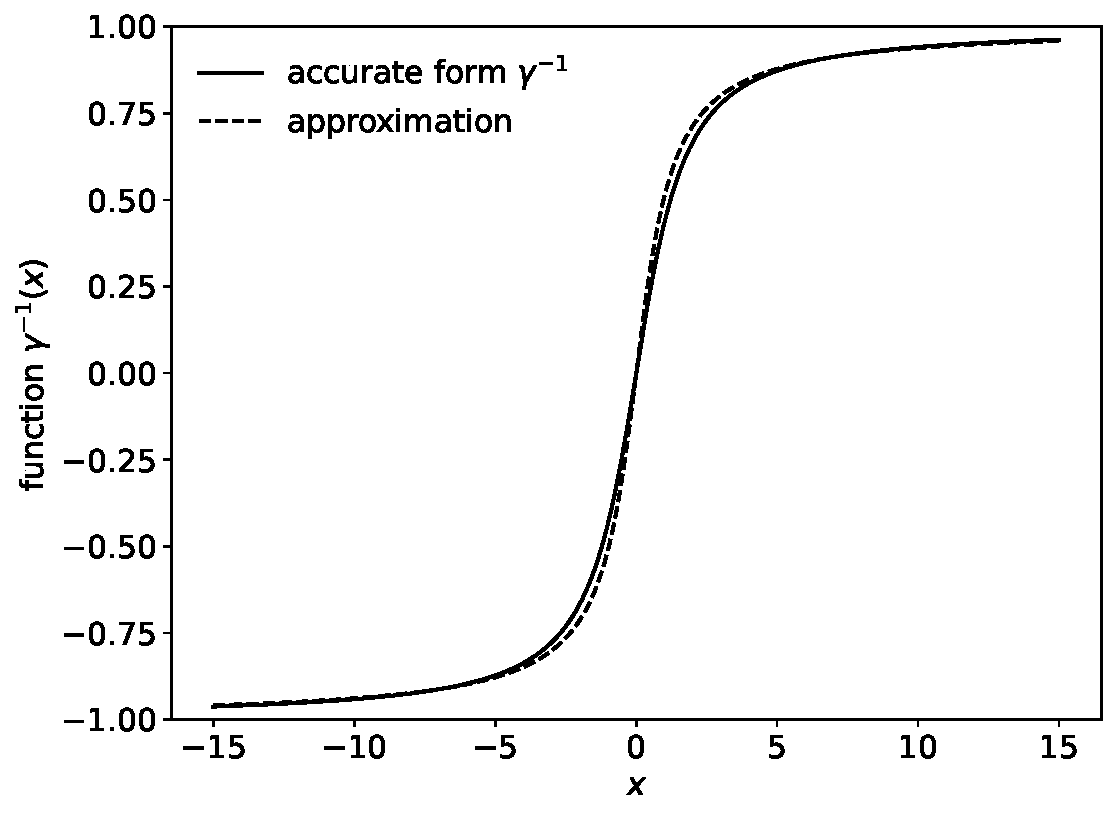
\includegraphics[width=\linewidth]{approx_invgamma.pdf}
        \caption{Auxiliary Function $\gamma^{-1}(x)$}
    \end{subfigure}
    \hfill
    \begin{subfigure}{0.48\textwidth}
        \centering
        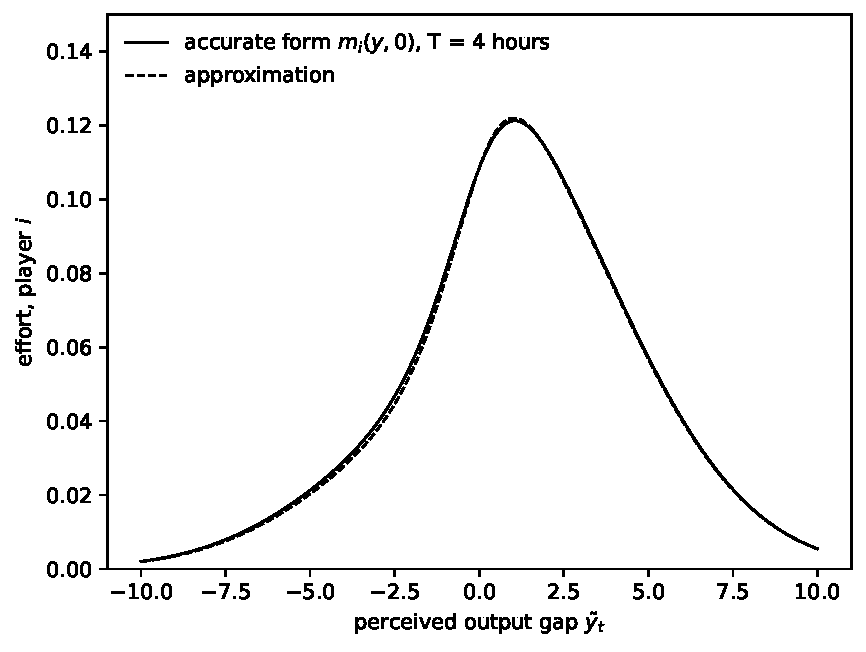
\includegraphics[width=\linewidth]{approx_equi_effort.pdf}
        \caption{Equilibrium Effort $m_i(\tilde{y}_t, t)$}
    \end{subfigure}
    \caption{Comparison of the Accurate and Approximate Forms ($\theta = 1$, $c_i = c_j = 1$, $\sigma=1$, $\Delta=1/24$)}
    \label{fig-approximation}
\end{figure}

In our Bayesian framework, we specify truncated normal distributions with large variances as priors for the unknown parameters $\Theta$.
This choice is intended to make the priors as uninformative as possible, thereby minimizing their influence on the posterior distribution. 
By allowing the parameters to vary broadly within reasonable bounds, these weakly informative priors let the data play a dominant role in shaping the inference, while still ensuring mathematical well-posedness and numerical stability.


The following lemma establishes the identifiability of the model parameters.

\begin{lemma}\label{lmm-params-identifiability}
The contest parameters $c_i$, $c_j$, $\sigma$, $\lambda$ and $\mu_0$ are jointly identifiable. 
\end{lemma}




\section{Synthetic Experiments}\label{sect-synthetic}

Before applying our estimation procedure to real-world contest data, we evaluate its potential on synthetically generated data. 
The use of synthetic data serves not only to validate the effectiveness of Bayesian inference, but also to enhance our understanding of the underlying data-generating process, which is summarized in Algorithm~\ref{algo-dgp}. 

\begin{algorithm}[H]
\caption{Synthetic Data Simulation}
\label{algo-dgp}
\begin{algorithmic}
\STATE \textbf{Input:} 
	$\Delta$, $T$, $c_i$, $c_j$, $\sigma$, $\lambda$, $r$, $\tau^\star$, $y_0$, $\mu_0$
\STATE Sample $\{s_k^{i(j)}\}^{N_{i(j)}}_{k=1}$ from Poisson process $(\tau^\star)$ on $[0, T)$
\STATE Sample $\{u_k^{i(j)}\}^{N_{i(j)}}_{k=1}$ from uniform distribution on $[0, 1]$
\STATE Sample series of Brownian motions $(W_t)$ and $(B_t)$
\STATE Initialize $\ell^{i(j)}=0$, $\hat{y}_0 = 0$, $\tilde{y}_t=\mu_0$
\FOR{$t = 0$ to $T$}
    \STATE $m_{i(j)}(\tilde{y}_t, t)$  $\gets$ (\ref{eq-equilibrium-effort}), $\tau^{i(j)}(t)$ $\gets$ (\ref{eq-model-intensity})
    \hfill \COMMENT{Use $\theta$, $c_{i(j)}$, $\sigma$, $r$, $T$}
    \STATE $y_{t+\Delta} \gets$ (\ref{eq-state-dynamics}); $\tilde{y}_{t+\Delta}$ $\gets$ (\ref{eq-fintered-y-update})
    \hfill \COMMENT{Use $\sigma$, $\lambda$, $\Delta$, $W_{t+\Delta}$, $y_0$}
    \FOR{$s_{k}^{i(j)} \in [t, t+\Delta)$} 
        \IF {$u_k^{i(j)} < \tau_{i(j)}(s_{k}^{i(j)}) / \tau^\star_{i(j)}$}
        	    \STATE $\hat{t}^{i(j)}_{\ell} \gets s_{k}^{i(j)}$; $\ell^{i(j)} \gets \ell^{i(j)}+1$
	    \hfill \COMMENT{Accept the submission event}
	    \STATE $\hat{y}_{t+\Delta} \gets $ (\ref{eq-leaderboard-gap})
	    \hfill \COMMENT{Use $\sigma$, $\lambda$, $B_{t+\Delta}$}
        \ENDIF
    \ENDFOR
\ENDFOR
\STATE \textbf{Output:} $(y_t)$, $(\tilde{y}_t)$, $(m_{i(j)}(\tilde{y}_t, t))$, $\{\hat{t}_k^{i(j)}\}^{N_{i(j)}}_{k=1}$, $(\hat{y}_{t_k})_{k=1}^{N_i + N_j}$
\end{algorithmic}
\end{algorithm}

A central challenge in generating synthetic data lies in dynamically constructing a point process that conforms to an inhomogeneous Poisson process.
We first generate candidate submission events according to a homogeneous Poisson process over the whole contest duration, using a fixed high intensity $\tau^\star \ge \sup_t \tau_{i(j)}(t)$.
Then, we apply the classical thinning procedure \citep{lewis1979simulation} to determine whether each candidate event is accepted or not.

As a concrete example, we consider an artificial contest that spans a three-month period, from January 1 to April 1, 2025.
The contest involves two participants, $i$ and $j$, who differ slightly in their effort costs.
Specifically, the unit costs of effort are set to $c_i = 1.2$ and $c_j = 1.5$, respectively. 
The innovation risk of the contest is assumed to be $\sigma = 2.0$, and the precision of the signal is set to $\lambda = 1.0$. 
The prize value $\theta$ is normalized to one. 
Additionally, we assume the ratio between submission intensity and effort is given by $r = 15$. 
Under this specification, we simulate the trajectory of the true output gap $(y_t)$, the submission times $\{t^i_k\}_{k=1}^{N_i}$ and $\{t^j_k\}_{k=1}^{N_j}$ for both players, and the corresponding updates to the public leaderboard $(\hat{y}_{t_k})_{k=1}^{N_i + N_j}$. 
We also compute the perceived output gap $(\tilde{y}_t)$ over time, as well as the equilibrium effort levels $(m_i(\tilde{y}_t, t))$ and $(m_j(\tilde{y}_t, t))$. 

\begin{figure}[!ht]
	\noindent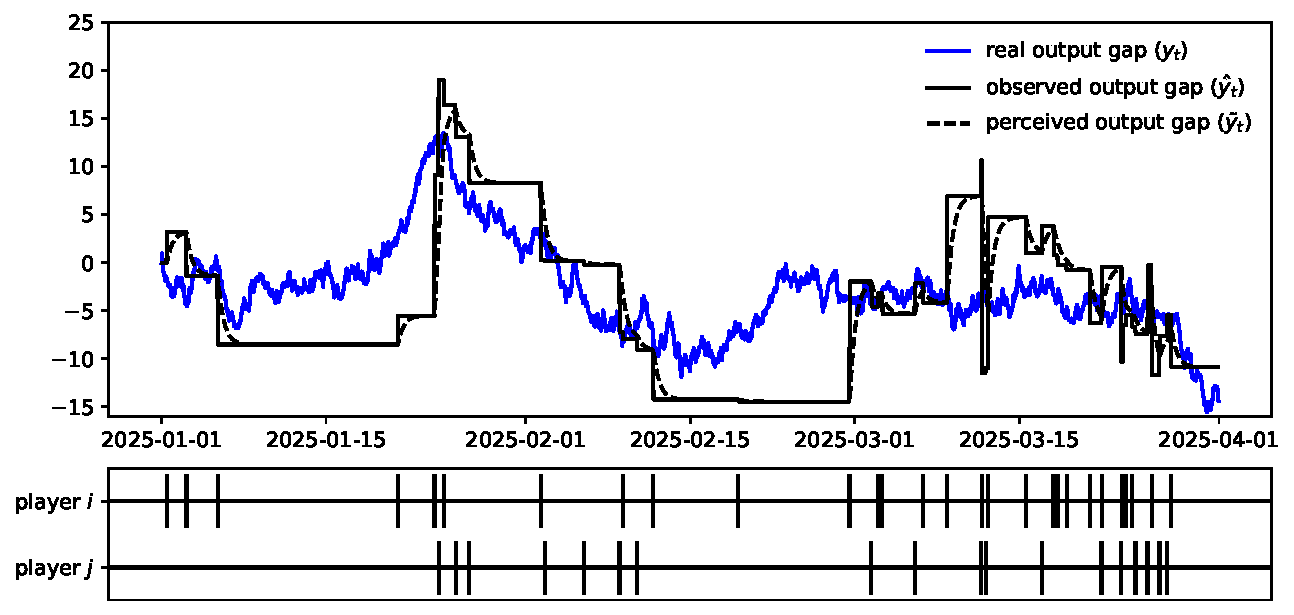
\includegraphics[scale=0.75]{synthetic_data.pdf}
	\caption{Synthetic Contest Data of Two Players from 2025-01-01 to 2025-04-01\\($\theta = 1.0$, $c_i = 1.2$, $c_j = 1.5$, $\sigma = 2.0$, $\lambda = 1.0$, $r = 15$)}
	\label{fig-synthetic_90}
\end{figure}

Figure~\ref{fig-synthetic_90} shows a realization of the virtual contest described above.
The blue line in Figure~\ref{fig-synthetic_90} represents the underline true output gap $y_t$, which can be interpreted as a \textit{private} leaderboard visible only to the contest designer, who has exclusive access to the full dataset.
Its drift is determined by the cumulative effort gap between the two players, while its volatility is governed by the contest’s innovation risk parameter $\sigma$. 
The solid black line depicts the corresponding \textit{public} leaderboard $\hat{y}_t$, which is updated whenever a submission is made by either player $i$ or $j$, as indicated by the short vertical ticks.
Intuitively, the more information is disclosed, the more closely the public leaderboard $\hat{y}_{t_k}$ approximates the true state $y_{t_k}$; the level of signal noise is controlled by the precision parameter $\lambda$.
The dashed black line shows the players’ perceived output gap $\tilde{y}_t$, as inferred from the public leaderboard and defined in equation~(\ref{eq-fintered-y-update}).
Submission times $\hat{t}^i_k$ and $\hat{t}^j_k$, marked by the short vertical ticks, are driven by each player’s effort level and are modelled as realizations of an inhomogeneous Poisson process.
There are 28 submissions from player $i$ and 18 submissions from player $j$. 

One might observe that, between two submissions $\hat{t}_{k}$ and $\hat{t}_{k+1}$, the estimate variance of the two players $S_t$ should increase over time rather than remain constant as we have assumed. 
However, under our modelling assumption where no submission implies low effort, a Bayesian player would infer that inactivity signals low intensity, thereby narrowing the estimation variance. 
For analytical tractability and to leverage the steady-state equilibrium formulation (\ref{eq-equilibrium-effort}), we abstract from modelling time-varying uncertainty.

Each parameter of $\Theta$ is assigned a truncated normal prior, with the choice of mean, variance, and support tailored to ensure numerical stability and to reflect the amount of prior information available.
Specifically, the prior distribution for each parameter $c_i$ and $c_j$ is specified as a truncated normal distribution bounded between 0.1 and 5, with a mean of 0.5 and variance of 5.
The prior for $\sigma$ follows a truncated normal distribution on the interval [0.5, 10], with mean 1 and variance 5.
Similarly, the prior for $\lambda$ supports on [1e-6, 10], also with mean 1 and variance 5.
The prior for $\mu_0$, by contrast, is more informative: it follows a truncated normal distribution over [-20, 20], centered at the observed initial value $\hat{y}_0$ with variance 1.
This reflects a stronger prior belief about the initial latent state and serves to anchor the model, thereby enhancing the stability and identifiability of the inference procedure.

\begin{table}[htbp]
\newcolumntype{Y}{>{\centering\arraybackslash}X}
\centering
\caption{Bayesian Estimates from Synthetic Data}\label{tbl-contest90}
\begin{tabularx}{\textwidth}{lYYYYY}
\toprule
\textbf{Parameters} & \textbf{$c_i$} & \textbf{$c_j$} & \textbf{$\sigma$} & \textbf{$\lambda$} & \textbf{$\mu_0$} \\
\addlinespace[0.25ex]
\cline{2-6}
\addlinespace[0.25ex]
(true val.)        & 1.2 & 1.5 & 2.0 & 1.0 & 0.0 \\
\midrule
 Posterior Mean    & 1.089 & 1.751 & 2.801 & 1.105 & 0.005 \\
 Posterior Stderr   & 0.258 & 0.476 & 0.503 & 0.299 & 0.990 \\
 RMSE                  & 0.281 & 0.538 & 0.945 & 0.317 & 0.990 \\
 95\% Interval        
		& [0.68, 1.68] 
		& [1.01, 2.85]
		& [1.95, 3.93]
		& [0.62, 1.78] 
		& [-1.92, 1.94] \\
\bottomrule
\addlinespace[0.5ex]
\end{tabularx}
\begin{minipage}{\textwidth}
{\footnotesize
\textit{Note:} (1) $\text{MSE}(\hat\theta) = \mathbb{E}(\hat{\theta}-\theta)^2 = [\mathbb{E}(\hat{\theta}) - \theta]^2 + Var(\hat{\theta})$ by the bias–variance decomposition. RMSE is then calculate by the squared root of MSE. 
(2) Players $i$ and $j$ submit 28 and 18 times respectively.
}
\end{minipage}
\end{table}

Table~\ref{tbl-contest90} presents the Bayesian inference results based on the synthetic data that we display in Figure~\ref{fig-synthetic_90}. 
Due to the limited data from the short contest duration, the posterior distribution of some parameters (such as $\sigma$ in this example) remains relatively far from the true value.
Nevertheless, given the limited sample size, the performance of Bayesian estimation is satisfactory. 
For most parameters (specifically $c_i$, $c_j$, $\lambda$ and $\mu_0$), the posterior means lie reasonably close to their true values.

We next examine whether Bayesian estimation improves with increasing data quantity.


\subsection{Asymptotic Properties}

With the synthetic contest data in place, it is important to ensure that our Bayesian framework is statistically coherent and implemented correctly. 
To this end, we numerically examine the asymptotic behaviour of the posterior distribution under two scenarios:
$i$) repeating the experiment multiple times under a fixed data-generating process, and $ii$) observing a single contest over an long time horizon.
As the amount of data increases, posterior consistency ensures that the Bayesian posterior concentrates around the true parameter values (\citealt{vaart1998asymptotic}, \citealt{ghosal2000convergence}, \citealt{pokern2013posterior}, \citealt{ramamoorthi2015posterior}).
While our analysis is simulation-based rather than theoretical, it provides evidence that the proposed likelihood formulation and inference procedure behave as expected in large-sample regimes.


\subsubsection{Replications.}

To begin, we investigate the asymptotic behavior of the posterior distribution when multiple independent realizations of the contest are observed. 
Multiple contests are independently simulated under identical parameters, with their data pooled to form a larger sample for Bayesian inference.
This setting corresponds to a replicated experimental design and allows us to assess whether Bayesian inference consistently recovers the true parameters as the number of observed contests increases.

The experimental results are presented in Table~\ref{tbl-pool-synthetic-data}. 
We replicate the contest simulation with 10 and 20 independent instances. 
Compared with Table~\ref{tbl-contest90}, we find that as the sample size increases, the RMSE of most parameters decreases, indicating that the posterior distributions converge more closely to the true parameter values.

\begin{table}[htbp]
\newcolumntype{Y}{>{\centering\arraybackslash}X}
\centering
\caption{Bayesian Estimates from Pooled Synthetic Data}\label{tbl-pool-synthetic-data}
\begin{tabularx}{\textwidth}{lYYYYY}
\toprule
\textbf{Parameters} & \textbf{$c_i$} & \textbf{$c_j$} & \textbf{$\sigma$} & \textbf{$\lambda$} & \textbf{$\mu_0$}\\
\addlinespace[0.25ex]
\cline{2-6}
\addlinespace[0.25ex]
(true val.)        & 1.2 & 1.5 & 2.0 & 1.0 & 0.0\\
\midrule
\addlinespace
\multicolumn{5}{l}{\textbf{Pool of 10 Contests}} \\
Posterior Mean  & 1.254 & 1.686 & 1.912 & 1.053 & -0.009\\
Posterior Stderr & 0.087 & 0.128 & 0.095 & 0.090 & 0.975\\
RMSE                & 0.102 & 0.225 & 0.130 & 0.104 & 0.975\\
\addlinespace
\multicolumn{5}{l}{\textbf{Pool of 20 Contests}} \\
Posterior Mean  & 1.204 & 1.639 & 1.981 & 0.988 & 0.008\\
Posterior Stderr & 0.060 & 0.089 & 0.068 & 0.060 & 1.003\\
RMSE                & 0.060 & 0.165 & 0.071 & 0.062 & 1.003\\
\bottomrule
\addlinespace[0.5ex]
\end{tabularx}
\begin{minipage}{\textwidth}
{\footnotesize
\textit{Note:} $\text{MSE}(\hat\theta) = \mathbb{E}(\hat{\theta}-\theta)^2 = [\mathbb{E}(\hat{\theta}) - \theta]^2 + Var(\hat{\theta})$ by the bias–variance decomposition. RMSE is then calculate by the squared root of MSE. 
}
\end{minipage}
\end{table}

%%%%%%%%%%%%%%%%%%%%%%%%%%%%%%%%%%%

\begin{table}[htbp]
\newcolumntype{Y}{>{\centering\arraybackslash}X}
\centering
\caption{Bayesian Estimates from Long Term Synthetic Data}\label{tbl-longterm-synthetic-data}
\begin{tabularx}{\textwidth}{lYYYYY}
\toprule
\textbf{Parameters} & \textbf{$c_i$} & \textbf{$c_j$} & \textbf{$\sigma$} & \textbf{$\lambda$} & \textbf{$\mu_0$}\\
\midrule
\multicolumn{5}{l}{\textbf{Contest of 6 Months}} \\
True Value           & 0.6     & 0.75   & 2.0     & 1.0     & 0.0\\
Posterior Mean    & 0.806 & 0.936 & 1.685 & 1.116 & 0.011\\
Posterior Stderr   & 0.112 & 0.142 & 0.148 & 0.171 & 0.986\\
RMSE                  & 0.234 & 0.234 & 0.348 & 0.207 & 0.986\\
\addlinespace
\multicolumn{5}{l}{\textbf{Contest of 12 Months}} \\
True Value           & 0.3     & 0.375 & 2.0     & 1.0     & 0.0\\
Posterior Mean    & 0.333 & 0.436 & 2.067 & 1.101 & 0.012\\
Posterior Stderr   & 0.027 & 0.046 & 0.097 & 0.138 & 0.994\\
RMSE                  & 0.043 & 0.076 & 0.118 & 0.171 & 0.994\\
\bottomrule
\addlinespace[0.5ex]
\end{tabularx}
\begin{minipage}{\textwidth}
{\footnotesize
\textit{Note:} (1) $\text{MSE}(\hat\theta) = \mathbb{E}(\hat{\theta}-\theta)^2 = [\mathbb{E}(\hat{\theta}) - \theta]^2 + Var(\hat{\theta})$ by the bias–variance decomposition. RMSE is then calculate by the squared root of MSE. 
(2) Players $i$ and $j$ submit 59 and 51 times in the 6-month contest, and 100 and 97 times in the 12-month contest, respectively.
}
\end{minipage}
\end{table}



\subsubsection{Long-Horizon Contest.}

We then turn to an alternative asymptotic regime in which a single contest instance is observed over a long time horizon. 
Rather than increasing the number of trajectories, we examine how the accumulation of submissions over a longer period improves inference accuracy. 

When generating long-horizon contest data, it is important to appropriately lower the effort costs $c_i$ and $c_j$ to ensure sustained effort from the contestants.
This is because effort levels are influenced by the remaining time until the deadline:
according to equation~(\ref{eq-equilibrium-effort}), the further away the deadline, the lower the equilibrium effort. 
Moreover, with volatility held constant, a long contest duration increases the likelihood that the true output gap undergoes a random walk to an unusually high level, potentially resulting in unexpected early success \citep{ryvkin2022fight}.
These factors may affect the quality of the generated data. 

Table~\ref{tbl-longterm-synthetic-data} presents simulations of contests lasting 6 and 12 months. 
In the 6-month contest, we set the unit effort costs to $c_i = 0.6$ and $c_j = 0.75$, resulting in 31 submissions from player $i$ and 40 from player $j$.
For the 12-month contest, the effort costs are reduced to $c_i = 0.3$ and $c_j = 0.375$, with players $i$ and $j$ submitting 143 and 182 times, respectively.
The posterior results show that longer contest durations and more frequent submissions lead to smaller RMSEs in the posterior distribution, indicating improved recovery of the true parameter values.




\section{Empirical Application}\label{sec-kaggle-application}

In this section, we apply our model to multiple real-world Kaggle contests to evaluate the structural validity of the proposed theoretical contest model in Section~\ref{contest-theory} and the Bayesian estimation framework in Section~\ref{sect-bayes-framework}. 

We select a set of representative competitions from the Meta-Kaggle dataset and, for each contest, identify two focal participants $i$ and $j$ based on criteria such as submission frequency, activity duration, and final ranking.\footnote{
...
}
Using their submission records and public leaderboard trajectories, we construct the observed data $\{t^i_k\}^{N_i}_{k=1}$, $\{t^j_k\}^{N_j}_{k=1}$ and $(\hat{y}_t)$ and perform Bayesian estimation for each of these contests under a unified prior specification.

To validate the model’s structural relevance, we then conduct a cross-contest analysis using information not incorporated in the Bayesian inference—namely, the \textit{private} leaderboard scores $(y_t)$. 
These scores, which reflect the true performance of each submission but remain hidden from players during the contest, serve as an \textit{ex post} benchmark for evaluating model accuracy.
Specifically, we implement a cross-validation strategy by deriving alternative estimates of the contest-specific parameters $\lambda$ and $\sigma$ from the private leaderboard data $(y_t)$ and comparing them to the structural estimates from our Bayesian procedure, thereby assessing the empirical explanatory power of the theoretical model.
Figure~\ref{kaggledata-diagram} provides a schematic representation of the data-model structure and the cross-validation strategy used to assess model validity.

\begin{figure}[!ht]
	\centering
	\noindent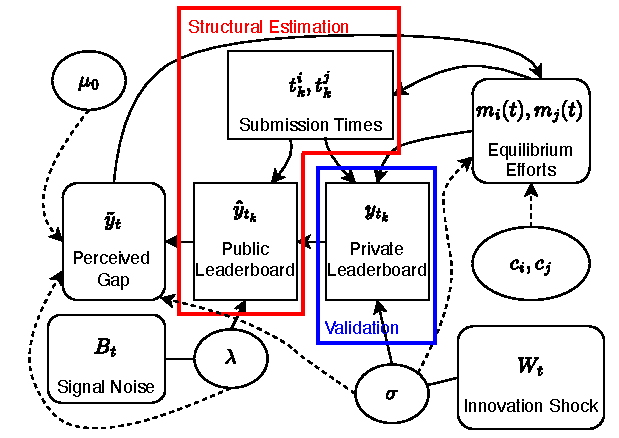
\includegraphics[scale=1.5]{kaggledata_diagram.pdf}
	\caption{Meta-kaggle Dataset Structure Diagram}
	\label{kaggledata-diagram}
	\begin{minipage}{\textwidth}
{\footnotesize
\medskip
\textit{Note:} (1) Rectangles, rounded rectangles and ellipses represent observed data, latent states and parameters, respectively. 
(2) Solid lines depict relationships among variables of time series data and state variables; dashed arrows show the influence of contest parameters. 
}
\end{minipage}
\end{figure}


\subsection{Mapping the Model to the Real Data}

To empirically implement the structural estimation developed in previous sections, we must first establish a clear mapping between the model’s theoretical components and the available real-world data. 
In particular, we describe how competitions are selected, how key players are identified, and how relevant contest-specific information—such as prize structures—is incorporated to reflect the incentives embedded in our model setup.


First, we restrict attention to Kaggle competitions that offer monetary prizes denominated in USD. 
Since our theoretical model focuses on winner-take-all contests, we prioritize competitions that award a single prize, i.e., reward number is equal to one. 
In practice, however, many contests distribute multiple prizes. 
For those awarding two or three prizes, we focus exclusively on the top two participants and treat the difference between the first- and second-place prize amounts as the effective reward for winning. 
This approach enables us to approximate a winner-take-all environment while retaining a sufficient number of real-world observations. 

Unlike in our model where the losing player receives nothing, non-winning Kaggle participants often gain symbolic recognition, such as medals. 
These additional incentives introduce noise that complicates the identification of a pure winner-take-all structure. 
By concentrating on the prize \emph{gap} between the top two players, we mitigate such confounding factors and better align the data with the competitive setting assumed in our model.

Next, we describe the procedure for selecting the two focal participants in each contest. 
We begin by examining the final rankings on the private leaderboard and consider candidates from the top downward. 
To ensure meaningful competition and sufficient data availability, we impose two selection criteria: (1) each participant must have submitted at least five times, and (2) the overlap in their active periods must exceed a minimum threshold. 
The first condition ensures that a participant appears frequently enough on the public leaderboard to attract the attention of potential competitors, while the second guarantees that the two players engaged in sustained competition over a sufficiently long time window. These requirements help ensure that the observed data is informative and that the contest dynamics are suitable for reliable Bayesian inference.

The practice of selecting only two participants from a larger pool of contestants may raise several potential concerns. First, it may limit the representativeness of the analysis by omitting the broader range of strategies exhibited by other participants. Second, reducing a multi-agent competition to a two-player setting might oversimplify the strategic complexity inherent in real-world contests. Third, choosing the top two players based on ex post rankings from the private leaderboard may introduce hindsight bias, thereby deviating from the model’s ex ante perspective. Finally, the presence of additional contestants could exert indirect influence on the focal pair’s behavior, complicating causal interpretation.

However, in the context of Kaggle competitions, several platform features help mitigate these concerns. Team compositions and individual profiles are publicly visible, and rich historical information—such as past rankings, medal counts, and shared code—allows participants to form credible beliefs about each other’s technical strength. The public leaderboard is updated frequently during the contest, enabling participants to track top-performing teams in real time. Moreover, Kaggle discussions and public notebooks foster an environment of semi-transparency, in which ideas, methods, and progress are often informally revealed. These factors enable top teams to recognize their closest rivals early and adjust their strategies accordingly. As a result, it is reasonable to assume that intense competition primarily arises among the strongest participants, justifying the empirical focus on the top two teams.

Actually, this approach relies on an implicit assumption: participants have a basic understanding of each other’s relative strength. 
In the context of Kaggle competitions, this assumption is reasonable. 
Team compositions are publicly available, and individual profiles include detailed historical records—such as past rankings, medal counts, and shared notebooks—that allow participants to quickly gauge the technical abilities of their competitors. 
Additionally, forum discussions and public notebooks create a semi-transparent environment where ideas and strategies are informally exchanged. 
These factors collectively enable top teams to identify potential competitors and adjust their strategies accordingly.





\subsection{Structural Validation}

...

To Do 1: relation between $\lambda$ and the proportion of data release?

By the data generating process (\ref{eq-leaderboard-gap}), we have a simple maximum likelihood estimation (MLE) of the true value of $\lambda$. 
Let $c = {1, 2, ..., N^c}$ index the contest.
Since $\hat{y}_t^c - y_t^c \sim \mathcal{N}(0, 1/(\lambda_c\Delta))$, we have 
\begin{equation*}
\lambda^{\text{MLE}}_c = \frac{N^c}{\Delta\sum^{N^c}_{k=1}(y_k^c - \hat{y}_k^c)^2}, \quad N^c = T/\Delta
\end{equation*}

Below is the regression result:

%%%%%%%%%% Figure & Table %%%%%%%%%%%
\noindent
\begin{minipage}[t]{0.43\textwidth}
	\vspace*{\fill}
	\centering
	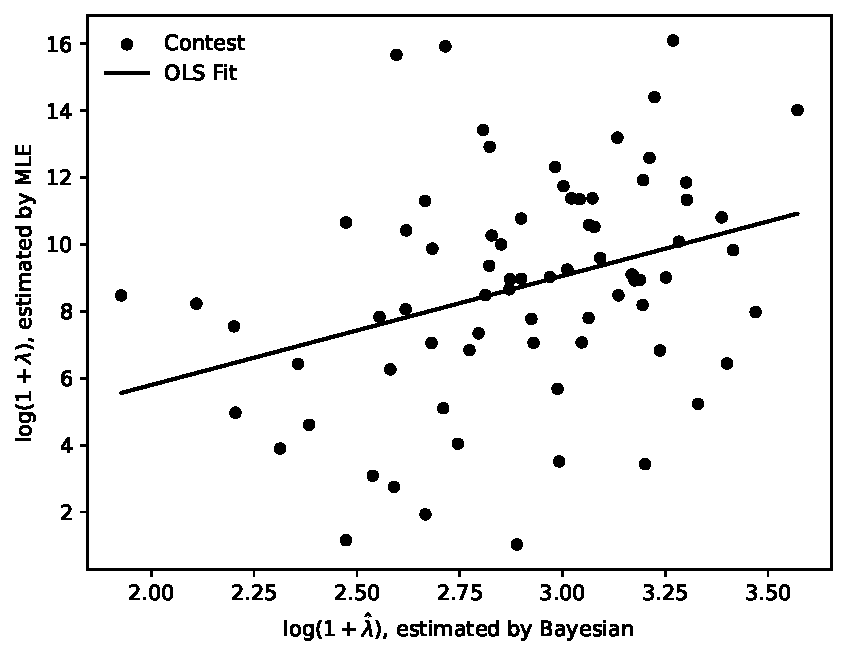
\includegraphics[width=\linewidth]{validate_lamb.pdf}
	\vspace*{\fill}
\end{minipage}
\hfill
\begin{minipage}[t]{0.53\textwidth}
	\vspace*{\fill}
	\centering
	\newcolumntype{Y}{>{\centering\arraybackslash}X}
	\begin{tabularx}{\textwidth}{llYY}
		\toprule
		& coef. & stderr & 95\% CI \\
		\midrule
		const.
		& -0.733 & 3.181 & [-7.073, 5.607] \\
		$\log(1 + \hat{\lambda})$ 
		& 3.264\textbf{**} & 1.088 & [1.096, 5.432] \\
		\midrule
		Obs. & \multicolumn{3}{c}{75} \\
		R$^2$ & \multicolumn{3}{c}{0.110} \\
		Adj. R$^2$ & \multicolumn{3}{c}{0.098} \\
		\bottomrule
		\addlinespace[0.5ex]
	\end{tabularx}
	\begin{minipage}{\textwidth}
{\footnotesize
\textit{Note:} (1) Significance levels: \textbf{***} $p < 0.001$, \textbf{**} $p < 0.01$, \textbf{*} $p < 0.05$. 
(2) Normality diagnostics: Omnibus = 0.378, Jarque-Bera = 0.071, Skewness = -0.042, Kurtosis = 3.126. 
(3) Other diagnostic statistics: Condition Number = 28.2, Durbin-Watson = 2.244.
}
	\end{minipage}
	\vspace*{\fill}
\end{minipage}
%%%%%%%%%%%% Captions %%%%%%%%%%%%
\noindent
\begin{minipage}[t]{0.43\textwidth}
	\centering
	\captionof{figure}{...}
\end{minipage}
\hfill
\begin{minipage}[t]{0.53\textwidth}
	\centering
	\captionof{table}{...}
\end{minipage}
\medskip

Result: significantly positively related. 

To Do 2: validate the estimation of $\sigma$?

By the dynamic of private leaderboard (\ref{eq-state-dynamics}), with the submission times of contest $c$ denoted by $\{t^c_k\}^{N^c}_{k=1}$, we have $y^c_{k+1} - y^c_{k} \sim \mathcal{N}\left(\int^{t_{k+1}}_{t_k}m^c_i(s) - m^c_j(s)ds, \sigma^2(t^c_{k+1}-t^c_k)\right)$ . 
Then, by (\ref{normal-mle-sigma}), we can estimate the parameters $\sigma$ using MLE: 
\begin{equation*}
\sigma^{\text{MLE}}_c = \left(\frac{1}{N^c}\sum_k\frac{\left[y^c_{t^c_{k+1}}-y^c_{t_k}-\int^{t^c_{k+1}}_{t^c_k}m^c_i(s) - m^c_j(s)ds\right]^2}{t^c_{k+1}-t^c_k}\right)^{1/2}
\end{equation*}
where $\hat{r}$ is the Bayesian estimate. 

\noindent
\begin{minipage}[t]{0.43\textwidth}
	\vspace*{\fill}
	\centering
	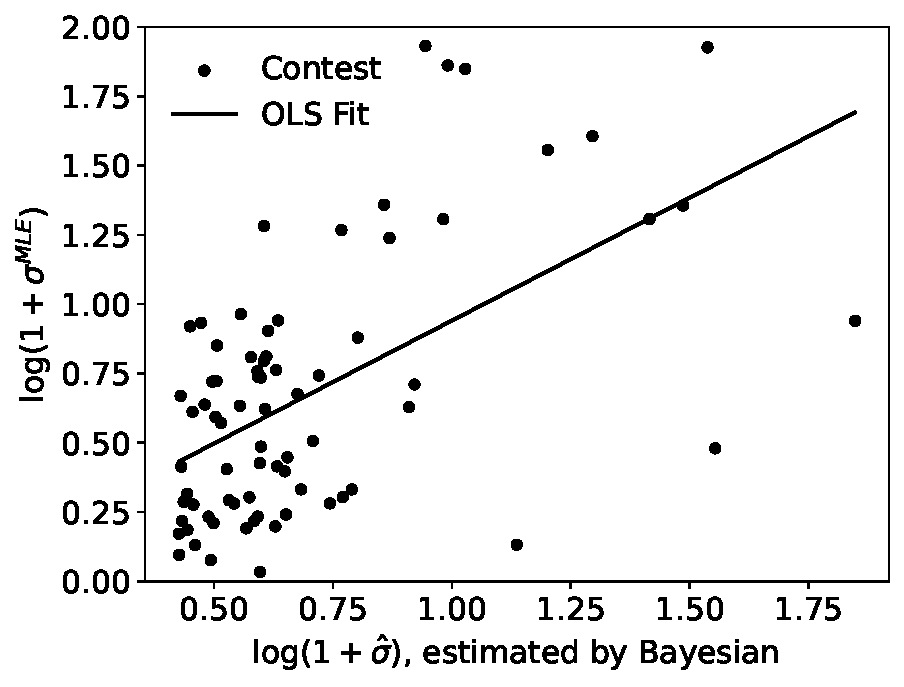
\includegraphics[width=\linewidth]{validate_sigma.pdf}
	\vspace*{\fill}
\end{minipage}
\hfill
\begin{minipage}[t]{0.53\textwidth}
	\vspace*{\fill}
	\centering
	\newcolumntype{Y}{>{\centering\arraybackslash}X}
	\begin{tabularx}{\textwidth}{llYY}
		\toprule
		& coef. & stderr & 95\% CI \\
		\midrule
		const.
		& 0.054 & 0.116 & [-0.178,0.285] \\
		$\log(1 + \hat{\lambda})$ 
		& 0.887\textbf{***} & 0.152 & [0.583, 1.190] \\
		\midrule
		Obs. & \multicolumn{3}{c}{75} \\
		R$^2$ & \multicolumn{3}{c}{0.317} \\
		Adj. R$^2$ & \multicolumn{3}{c}{0.308} \\
		\bottomrule
		\addlinespace[0.5ex]
	\end{tabularx}
	\begin{minipage}{\textwidth}
{\footnotesize
\textit{Note:} (1) Significance levels: \textbf{***} $p < 0.001$, \textbf{**} $p < 0.01$, \textbf{*} $p < 0.05$. 
(2) Normality diagnostics: Omnibus = 1.280, Jarque-Bera = 0.774, Skewness = 0.225, Kurtosis = 3.214.
(3) Other diagnostic statistics: Condition Number = 5.08, Durbin-Watson = 1.618.
}
	\end{minipage}
	\vspace*{\fill}
\end{minipage}
%%%%%%%%%%%% Captions %%%%%%%%%%%%
\noindent
\begin{minipage}[t]{0.43\textwidth}
	\centering
	\captionof{figure}{...}
\end{minipage}
\hfill
\begin{minipage}[t]{0.53\textwidth}
	\centering
	\captionof{table}{...}
\end{minipage}
\medskip

Result: significantly positively related. 

\section{Conclusion}

...

% Appendix here
% Options are (1) APPENDIX (with or without general title) or
%             (2) APPENDICES (if it has more than one unrelated sections)
% Outcomment the appropriate case if necessary
%
% \begin{APPENDIX}{<Title of the Appendix>}
% \end{APPENDIX}
%
%   or
%
% \begin{APPENDICES}
% \section{<Title of Section A>}
% \section{<Title of Section B>}
% etc
% \end{APPENDICES}


\newpage
\begin{APPENDICES}


\section{Proofs}

\proof{Proof of Lemma~\ref{lmm-params-identifiability}}
Suppose $\Theta = (c_i, c_j, \sigma, \lambda)$ and $\Theta' = (c'_i, c'_j, \sigma', \lambda')$. 
To show that the model parameters are jointly identifiable, it suffices to show that $\mathcal{L}(\hat{t}^i_k, \hat{t}^j_k, \hat{y}_k | \Theta) = \mathcal{L}(\hat{t}^i_k, \hat{t}^j_k, \hat{y}_k | \Theta')$ $\Rightarrow$ $\Theta = \Theta'$. 
\Halmos
\endproof



\section{Extensions}

\subsection{Staggered Entry of Multiple Players}
\label{sect-extension}

We index the participating teams of the contest by $i\in\{1, 2, ..., n\}$. 
To fully leverage the potential of the data and establish a connection with our theoretical model, let's assume that each participant perceives a competitor they are playing against at every moment, denoted as $j$. 
This perceived competitor is typically understood as the most prominent individual on the leaderboard, i.e., the person ranked first.
When team $i$ themselves hold the top position, their perceived competitor is the individual who poses the greatest threat, namely the person ranked second.

\subsection{Hybrid Kalman Filter}
\label{sect-kalman-filter}

% Submission
Let' suppose the submission events of the representative player $i$ occur at times $(t^i_1, t^i_2, ...)$ following an inhomogeneous Poisson process driven by the intensity function $\tau_i(t)$. 

% Signal
After each submission, the contest designer emits a \textit{public} signal of the real output $x_{i,t_k}$. 
The signal is ambiguous and the game holder controls the ambiguity. 
The dynamic of signal is 
\begin{equation}\label{signal}
	\hat{x}_{i,k} = x_{i,t_k} + \frac{v_{i,k}}{\sqrt{\lambda}}, \quad k=1, 2, ...
\end{equation}
where $v_{i,k}$ follows standard normal distribution and is independent with $(W_{i,t})$ and $(W_{j,t})$, and the parameter $\lambda$ is set by the game holder to control the precision of signals. 
The larger the $\lambda$, the more accurate the signal would be. 

% Bayesian Player
The information set of both players at time $t \ge 0$ is  $I_{t} := \{\hat{x}_{i,k}, \hat{x}_{j,k} : 0\le t_k \le t\}$. 
Both players estimate the unknown outputs $x_{i,t}$ and $x_{j,t}$ purely based on the information set $I_t$ and hidden actions $q_{i,t}$ and $q_{j,t}$. 
Let $\tilde{x}_{i,t} \equiv E(x_{i,t}|I_t)$ be the estimated output gap and $S_{i,t} \equiv E[(\tilde{x}_{i,t}-x_{i,t})^2|I_t]$ be the estimation variance. 
The conditional distribution $y_{t}|I_t\sim\mathcal{N}(\tilde{y}_{t},S_{t}|I_t)$ is fully captured by the mean $\tilde{y}_{t}$ and variance $S_{t}$. 

The evolution of $\tilde{x}_{i,t}$ and $S_{i,t}$ is characterized by a continuous-discrete Kalman Filter (CD-KF, \citealt{barrau2017invariant}, \citealt{frogerais2012various}), with the measurement of each step $k=1, 2, ...$ consisting of two phases: in
(1) prediction phase during time interval $(t_{k-1}, t_{k})$, equations are derived from those of Kalman-Bucy filter \citep{Bensoussan1992Control} without considering the Kalman gain: 
\begin{align}
	d\tilde{x}_{i,t} &= q_{i,t}dt
	\label{filtered-x}\\
	dS_{i,t} &= \sigma^2dt
	\label{filtered-S}
\end{align} 
and in (2) updation phase $t=t_k$, equations are 
\begin{align}
	\tilde{x}_{i,k}^{+} &= \tilde{x}_{i,k}^{-} + \frac{\lambda S_{i,t_k}^{-}}{\lambda S_{i,t_k}^{-}+1}\left(\hat{x}_{i,k} - \tilde{x}_{i,t_k}^{-}\right)
	\label{updated-x}\\
	S_{i,t_k}^{+} &= \frac{S_{i,t_k}^{-}}{\lambda S_{i,t_k}^{-}+1} 
\end{align}
If $\lambda = 0$, we have $S_t = S_0+\sigma^2t$, i.e., the estimation variance is increasing in time linearly. 
If $\lambda > 0$, the estimation error decreases after each update of the public leaderboard, i.e., $S_{i,t_k}^+ < S_{i,t_k}^-$. 



\section{Auxiliary Results}

\subsection{Solve $S_t$ in Equation (\ref{filtered-S})}\label{app-S-equ}

If $S$ is in steady state $dS/dt = 0$ $\Leftrightarrow$ $S = \bar{S} \equiv \sigma/\sqrt{\lambda}$. 
If $S$ is not in steady state, i.e. $S\not=\bar{S}$, we first isolate the two variables and get 
\begin{equation*}
	\frac{dS}{\sigma-\lambda S^2} = dt
\end{equation*}
Then, we take the integral on both sides
\begin{equation*}
    t = \int \frac{dS}{\sigma-\lambda S^2} = \frac{1}{\sigma\sqrt{\lambda}} \int \frac{dS\sqrt{\lambda}/\sigma}{1 - (S\sqrt{\lambda}/\sigma)^2} \equiv \frac{1}{\sigma\sqrt{\lambda}}\int \frac{du}{1-u^2} 
\end{equation*}
where $u = S\sqrt{\lambda}/\sigma = S/\bar{S}$. Hence, 
\begin{equation*}
    \sigma\sqrt{\lambda}\cdot t = \begin{cases}
        \tanh^{-1}(u)-K_1, & \text{if } |u|<1\\
        \coth^{-1}(u)-K_2, & \text{if } |u|>1
    \end{cases} = \begin{cases}
        \tanh^{-1}(S/\bar{S})-K_1, & \text{if } S<\bar{S}\\
        \coth^{-1}(S/\bar{S})-K_2, & \text{if } S>\bar{S} 
\end{cases}
\end{equation*}
Thus, we conclude the non-steady state case that 
\begin{equation*}
	S = \begin{cases}
		\bar{S}\cdot\tanh(\sigma\sqrt{\lambda}\cdot t + K_1), & \text{if } S<\bar{S}\\
		\bar{S}\cdot\coth(\sigma\sqrt{\lambda}\cdot t + K_2), & \text{if } S>\bar{S} 
	\end{cases}
\end{equation*}
Finally, we determine the constants $K_1$, $K_2$ by the initial condition $S_0$ and have 
\begin{align*}
	K_1 &= \tanh^{-1}(S_0/\bar{S})\\
	K_2 &= \coth^{-1}(S_0/\bar{S})
\end{align*}


\subsection{MLE for $r$ and $\sigma^2$}

Suppose we observe independent data points \( X_1, ..., X_n \), where each \( X_k \sim \mathcal{N}(M_k / r, \sigma^2 T_k) \) with known constants \( M_k \) and \( T_k \). 
The goal is to estimate the parameters \( r \) and \( \sigma \) via maximum likelihood estimation (MLE).
Ignoring constant terms, the log-likelihood function of the observed data is
\[
\ell(r, \sigma^2) = - \frac{n}{2} \log(\sigma^2) - \frac{1}{2\sigma^2} \sum_{k=1}^n \frac{\left( X_k - M_k/r \right)^2}{T_k}.
\]
To estimate $r$, we expand the summation of second term and have 
\[
Q(r) = \sum_{k=1}^n \left( \frac{X_k^2}{T_k} - \frac{2X_k M_k}{r T_k} + \frac{M_k^2}{r^2 T_k} \right)
= A - \frac{2B}{r} + \frac{C}{r^2},
\]
where \( A = \sum X_k^2/T_k \), \( B = \sum X_k M_k/T_k \), and \( C = \sum M_k^2/T_k \). Taking the derivative with respect to \( r \) and setting it to zero gives:
\begin{equation}\label{normal-mle-r}
\frac{dQ}{dr} = \frac{2B}{r^2} - \frac{2C}{r^3} = 0 \quad \Rightarrow \quad \hat{r} = \frac{C}{B} = \frac{\sum M_k^2/T_k}{\sum X_k M_k/T_k}.
\end{equation}
Then, substituting \( \hat{r} \) back into the likelihood, the MLE for \( \sigma^2 \) is obtained by maximizing
\[
\ell(\sigma^2) = -\frac{n}{2} \log(\sigma^2) - \frac{1}{2\sigma^2} \sum_{k=1}^n \frac{\left( X_k - M_k/\hat{r} \right)^2}{T_k},
\]
which yields
\begin{equation}\label{normal-mle-sigma}
\hat{\sigma}^2 = \frac{1}{n} \sum_{k=1}^n \frac{\left( X_k - M_k/\hat{r}\right)^2}{T_k}.
\end{equation}











\end{APPENDICES}



% Acknowledgments here
%\ACKNOWLEDGMENT{......}


% References here (outcomment the appropriate case)

% CASE 1: BiBTeX used to constantly update the references
%   (while the paper is being written).
%\bibliographystyle{informs2014} % outcomment this and next line in Case 1
%\bibliography{<your bib file(s)>} % if more than one, comma separated

% CASE 2: BiBTeX used to generate mypaper.bbl (to be further fine tuned)
%\input{mypaper.bbl} % outcomment this line in Case 2

%If you don't use BiBTex, you can manually itemize references as shown below.


%\bibliographystyle{nonumber}
\bibliographystyle{informs2014}
\bibliography{_Literatures.bib}

%%%%%%%%%%%%%%%%%
\end{document}
%%%%%%%%%%%%%%%%%
